We implemented kcores method
and tested other algorithms that are already implemented in the system with unit tests and other datasets from SNAP.

Figures below give the degree distribution and pagerank result of two dataset from SNAP. We can find that the degree distribution and pagerank results are consistent with the power law as nodes or pages with higher degree or rank have a small number while nodes or pages with lower degree or rank have a large number.
You can also find the detailed results in the output folder, which contains csv files for the results of belief propagation, connected components, node degrees, degree distribution, eigen values, k-core connected components, pagerank results, radius, etc. 


\begin{figure}[H]
\begin{center}
\begin{tabular}{cc}
     % uncomment the next lines, and give the right ps files
     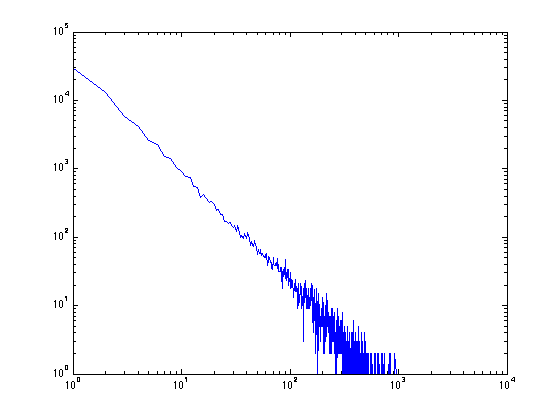
\includegraphics[width=0.3\textwidth]{FIG/soc-degreedist.png} &
     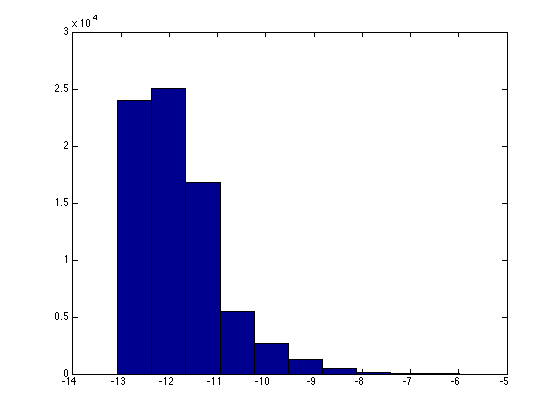
\includegraphics[width=0.3\textwidth]{FIG/soc-pagerank.png} \\
\end{tabular}
\caption{Degree Distribution(a) and PageRank(b) for Dataset SOC-Epinions1}

\begin{tabular}{cc}
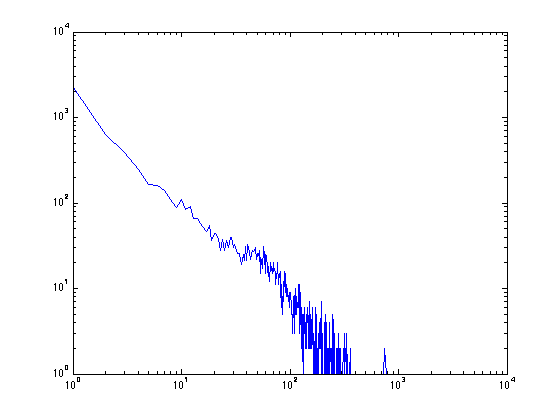
\includegraphics[width=0.3\textwidth]{FIG/wiki-degreedist.png} &
     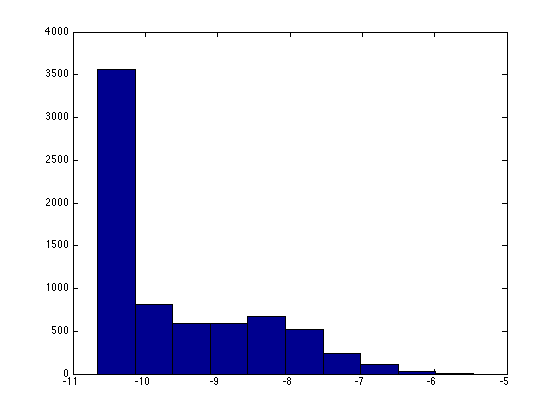
\includegraphics[width=0.3\textwidth]{FIG/wiki-pagerank.png} \\

     %\psfig{figure=FIG/plot.ps,width=2in} \\
     % \psfig{figure=FIG/data.ps,width=2in} &
     % \psfig{figure=FIG/plot.ps,width=2in} \\
    (a) & (b)
\end{tabular}
\caption{Degree Distribution(a) and PageRank(b) for Dataset wiki-Vote}

\end{center}
\end{figure}

The figures below also include the degree distribution, connected components, k=5 cores algorithm results on the 5 unit tests.
As the unit tests are small, there is no nodes in the tests that satisfy k=5 cores, so the output result for these 5 
unit tests are empty. 
However, you can find the node id, component id pairs in the stdout output from console or in the kcorecomponent.csv file, which shows that the k-core
algorithm works as it claims to find correct coreness subgraphs.

\begin{figure}[H]
\begin{center}
\begin{tabular}{cc}
     % uncomment the next lines, and give the right ps files
     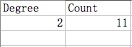
\includegraphics[width=0.3\textwidth]{FIG/1dd.jpg} &
     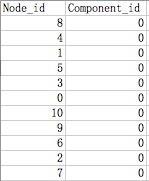
\includegraphics[width=0.3\textwidth]{FIG/1cc.jpg} \\
\end{tabular}
\caption{Degree Distribution(a), connected components(b) for Dataset1}
\end{center}
\end{figure}

\begin{figure}[H]
\begin{center}
\begin{tabular}{cc}
     % uncomment the next lines, and give the right ps files
     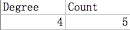
\includegraphics[width=0.3\textwidth]{FIG/2dd.jpg} &
     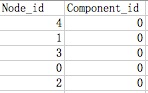
\includegraphics[width=0.3\textwidth]{FIG/2cc.jpg} \\
\end{tabular}
\caption{Degree Distribution(a), connected components(b) for Dataset2}
\end{center}
\end{figure}

\begin{figure}[H]
\begin{center}
\begin{tabular}{cc}
     % uncomment the next lines, and give the right ps files
     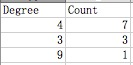
\includegraphics[width=0.3\textwidth]{FIG/3dd.jpg} &
     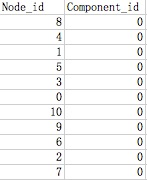
\includegraphics[width=0.3\textwidth]{FIG/3cc.jpg} \\
\end{tabular}
\caption{Degree Distribution(a), connected components(b) for Dataset3}
\end{center}
\end{figure}

\begin{figure}[H]
\begin{center}
\begin{tabular}{cc}
     % uncomment the next lines, and give the right ps files
     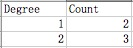
\includegraphics[width=0.3\textwidth]{FIG/4dd.jpg} &
     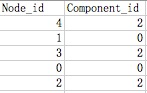
\includegraphics[width=0.3\textwidth]{FIG/4cc.jpg} \\
\end{tabular}
\caption{Degree Distribution(a), connected components(b) for Dataset4}
\end{center}
\end{figure}

\begin{figure}[H]
\begin{center}
\begin{tabular}{cc}
     % uncomment the next lines, and give the right ps files
     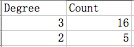
\includegraphics[width=0.3\textwidth]{FIG/5dd.jpg} &
     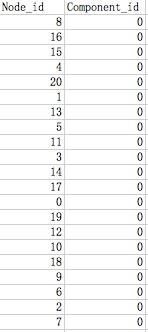
\includegraphics[width=0.3\textwidth]{FIG/5cc.jpg} \\
\end{tabular}
\caption{Degree Distribution(a) connected components(b) for Dataset5}
\end{center}
\end{figure}
